\section{PCE Maps} 
\subsection{Quantum channels} % {{{
Quantum channels comprehend the most general linear operations that a quantum
system undergo independently of its past~\cite{zimansbook,cirac}. To introduce
their construction and properties, first let us define several objects. We will
denote Hilbert spaces as \hilbert and $d$-dimensional Hilbert spaces as
$\hilbert_d$. The set of bounded operators over a Hilbert space \hilbert will
be written as $\mcB(\hilbert)$, the subset of density matrices as
$\mcS(\hilbert)$, which is in turn a subset of the so called trace-class
operators $\mcT(\hilbert)$, for the finite dimensional case, the one studied
here, $\mcT(\hilbert)$ and $\mcB(\hilbert)$ coincide~\cite{zimansbook}. 

The construction of quantum channels includes basically three ingredients:
linearity, trace preserving and complete positivity. The first one is needed to
send convex combinations of density matrices into the convex combination of the
evolution of such density matrices, this is, let $\mcE$ such linear operation,
thus $p \rho_1 +(1-p) \rho_2 \mapsto p \mcE[\rho_1]+(1-p)\mcE[\rho_2]$. The
trace preserving is required for the process $\mcE$ to be deterministic, this
is, $\tr\mcE[\rho]=\tr \rho =1$ is the probability that the process $\mcE$ will
happen to the state $\rho$, with $\rho \in \mcS(\hilbert)$. The complete
positivity condition is needed to preserve positive semidefiniteness and handle
the non-local character of quantum theory. This is, with positivity of the map
$\mcE$ one has $\mcE[\Delta]\geq 0 \ \ \forall \Delta \in \mcB(\hilbert)$ with
$\Delta\geq 0$. In the other hand, complete positvity of $\mcE$ reads $\id_k
\otimes \mcE[\omega]\geq 0$ for $k=1,2,\dots$, where $\omega$ is the Bell state
between the system and an ancilla with Hilbert space $\hilbert_k$. Therefore,
complete positivity ensures that every positive semidefinite operator of any
extension of the system (where the quantum channel is now a local operation) is
mapped into positive semidefinite operators, trace preserving is automatically
fulfilled for all extensions if $\mcE$ is. Thus, any density matrix of a system
where $\mcE$ acts locally, is sent to a valid density matrix, this is the
substance of complete positivity.

Quantum channels can be characterized by means of the Choi-\jami{} isomorphism~\cite{choi,jamil}. This is, given a linear operation $\mcE:\mcB(\hilbert)\to \mcB(\hilbert)$, the so-called Choi matrix of it, $C_\mcE=\left(\id \otimes \mcE\right)[\proj{\Omega}{\Omega}]$, where $\ket{\Omega}=1/\dim(\hilbert)\sum_i^{\dim(\hilbert)}\ket{i}\ket{i}$ is the Bell state between to copies of \hilbert, is positive semi-definite if and only if $\mcE$ is completely positive.

Quantum channels have the well-known \textit{Kraus representation} (or operator-sum representation) which reads $\mcE[\rho]=\sum_i K_i \rho K^\dagger{}_i$ in fact, a linear operation is completely positive if and only if it has a Kraus representation [cite Kraus book]

  \ddnote{[Choi representation, Kraus operators and Stinespring
dilation]}

It can be seen from Kraus decomposition that quantum channels preserve hermiticity, this has a practical consequence when using hermitian bases. $\hat \mcE_{ij}=\tr\left( \Delta_i \mcE[\Delta_j]
 \right)$

% }}}
\subsection{Single qubit case} % {{{
\label{sec:single:qubit}
\todo{David escribe una primera version y luego Carlos itera}
Let us discuss the single qubit case of \pce{} maps, they are defined by its action over Bloch vectors, providing that
\begin{equation}
\rho=\frac{\one +\vec r \cdot \vec \sigma}{2},
\end{equation}
then they are defined as follows
\begin{equation}
r_i \mapsto \tau_i r_i
\end{equation}
where $\tau_k$ is either $1$ or $0$. A direct evaluation of the 

 These operations have been studied in \cite{Ziman2005,davalosdivisibility} and are by definition diagonal in the Pauli basis $1/\sqrt{2} \left\{ \one, \sigma_x,\sigma_y,\sigma_z \right\}$, \ie{} $\hat \mcE=\diag{\left(1,\tau_x, \tau_y, \tau_z \right)}$. They form a tetrahedron in the space of eigenvalues 
 
with
\begin{equation}
\mcL_\alpha[\Delta]:= \frac{\gamma}{2}\left( \sigma_\alpha \Delta \sigma_\alpha -\Delta \right).
\label{eq:1qubit_semigroup}
\end{equation}
We will show later that this can be trivially generalized to the $N$ qubit case.



\begin{align}
U_\alpha\ket{\psi} \ket{0}:=\frac{1}{\sqrt{2}} \left( \ket{\psi} \ket{0}+\sigma_\alpha \ket{\psi}\ket{1} \right)\\
U_\alpha\ket{\psi} \ket{1}:=\frac{1}{\sqrt{2}} \left( \ket{\psi} \ket{0}-\sigma_\alpha \ket{\psi}\ket{1} \right)
\label{eq:1qubit_stinespring}
\end{align}
similar to the semigroup generator, we will show later that this can be trivially generalized to the $N$ qubit case.


\begin{itemize}
\item The single qubit case, describe some of the features.
\item Single qubit Kraus operators.
\item Single qubit relation with decoherence. 
\end{itemize}
% }}}
\subsection{Pauli component erasing maps} % {{{

\begin{itemize}
\item Canales de Ruskai Pauli maps, que la interseccion es no trivial (no estan contenidos en ninguna direccion, pero la interseccion es no vacia)
y Relación con canales citados en \cite{Siudzinska2020}? \cpnote{Esto quiza lo tengamos
que mover si es que necesitamos herramientas que discutiremos mas adelante para
hacer notar la diferencia}
\end{itemize}

The density matrix $\rho$ of a system of $N$ qubits can be written in Pauli
matrices basis as 
\begin{equation}\label{eq:N_qubits_rho}
	\rho =\frac{1}{2^N} 
            \sum_\valpha r_\valpha \sigma_\valpha,
%             \quad r_{\vec0}=1,
% 	\sigma_{\alpha_1}\otimes \ldots \otimes \sigma_{\alpha_N},
%             \sum_{\alpha_1,\ldots,\alpha_N=0}^3 \paulicomponents
% 	\sigma_{\alpha_1}\otimes \ldots \otimes \sigma_{\alpha_N},
	%r_{0,\ldots,0}=1,
\end{equation}
where $\vec \alpha$ denotes a vector index $\qty(\alpha_1,\ldots,\alpha_N)$,
$\sigma_{\vec \alpha} := \sigma_{\alpha_1}\otimes \ldots \otimes
\sigma_{\alpha_N}$ is the tensor product of Pauli matrices, and 
$r_{\vec \alpha}$ is the coefficient corresponding to the expansion
of the density matrix in the complete orthonormal basis $\left\{ 2^{-N/2}\sigma_{\vec
\alpha} \right\}$. In the sum each of the $N$ components of $\valpha$, i.e.
$\alpha_{1,\cdots,N}$ is varied from $0$ to $3$. 
Notice that $\sigma_{\vec 0} = \openone$, and since both $\tr \rho=1$ and 
$\tr \sigma_\valpha=2^N\delta_{\valpha,\vec 0}$, then $r_{\vec 0}=1$. 
We shall refer to $\paulicomponents$ as the ``Pauli components'' of the density
matrix of a system of qubits. 


%  $r_{\vec \alpha} =  $
% where $r_{0,\ldots,0}=1$ ($\Tr\rho=1$) and $\sigma_0=\openone$.


Consider the linear operations that simply attenuate the Pauli components of 
a multiqubit system:
\begin{equation}
	\paulicomponents \mapsto \taus \paulicomponents.
% 	\taus = 0,1, \hspace{1.5cm}	\tau_{0,\ldots,0}=1.
\end{equation}
These operations are diagonal in the basis $\left\{ 2^{-N/2}\sigma_{\vec \alpha} \right\}$, this follows straightforwardly from \eref{eq:sigma_property}, in fact, the diagonal components are exactly $\taus$, this is $\hat \mcE=\diag(\taus)$. Additionally, they are unital (leave invariant the complete mixture), in fact, as we will show later, they belong to the subset of unital channels that can be written as convex combinations of unitary channels.
 \cpnote{davalos, dale aca un pequeño rollo relevante quiza de una o dos
frases. También debemos tener un nombre pues lo de la diagonazliación funciona
para eso y quizá también seran relevantes para la parte de decoherencia}
\ddnote{De momento no he encontrado alguna reference, para qubits si, pero para
los generales no, estoy checando de nuevo el paper de Ruskai para entender que
tanto se solapan, a ver si puedo decir algo}.
For the operation to preserve the trace of the density matrix, we require that 
$\tau_{\vec 0}=1$. 
A Pauli component erasing (PCE) operation is a Pauli diagonal operation
%  A linear operation 
% $\mcE$ 
that either preserves or completely erases the Pauli components of a
density matrix. That is, 
% it transforms its Pauli components as 
\begin{equation} \label{eq:PCE_definition}
% \begin{split}
% 	\paulicomponents \mapsto \ \taus \paulicomponents,\hspace{.5cm}\\
% 	\taus = 0,1, \hspace{1.5cm}	\tau_{0,\ldots,0}=1.
	\paulicomponents \mapsto \taus \paulicomponents,\quad 
	\taus = 0,1.
% \end{split}
\end{equation}
It is worth noticing that not all PCE maps are quantum operations. For single 
qubits, if just one of the $\taus=0$, the complete positivity condition 
is not met, as discussed in \sref{sec:single:qubit}. It will be of central interest
in this article to determine which $\taus$ lead to a valid quantum map.

%\ddnote{hay un typo en esta ecuacion}
% A PCE operation is a trace-preserving operation that leaves invariant or erases 
% the Pauli components of a density matrix of $n$ qubits. \janote{Ojo que aquí 
% habrá que unificar la notación de subíndices. No lo hago porque no lo tengo del 
% todo claro y no hay problema en dejarlo así por el momento.}
% \cpnote{Aca voy} 

A graphical representation for PCE maps may be introduced, being the
two qubits case what has proved to be the most useful. Consider a $N$ dimensional 
Cartesian grid, with $4^N$ places.  Each place has $N$ integer coordinates, ranging
from 0 to 3, so each place corresponds to a given $\vec \alpha$ in 
\eref{eq:N_qubits_rho}. For a given PCE, we shall fill with black 
the corresponding position \cpnote{No me pone feliz esta redaccion}
if the corresponding $\tau_{\vec \alpha}=1$. Otherwise, we leave it 
empty. Examples for $N=1$ are provided in \fref{fig:one:qubit:examples}, whereas
for two qubits, we exemplify them in \fref{fig:two:qubit:examples}. 
% Notice
% than in both cases we drop the label $\alpha$ for simplicity, as it will 
% remain unchanged throughout this text \janote{No entiendo qué estás diciendo
% aquí}. 

\begin{figure} % {{{
\begin{center}
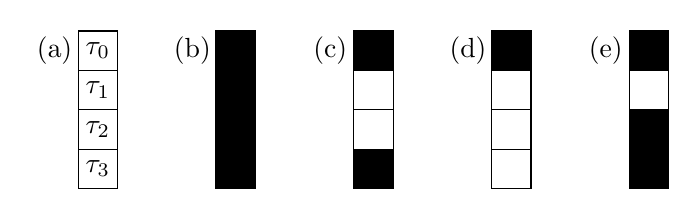
\begin{tikzpicture}[x=0.5cm, y=0.5cm] % {{{
\pgfmathsetmacro{\unitstep}{3.5}
% Coordenadas   {{{
\node at (-0.6,0.5) {(a)} ;
\draw (0,0) rectangle (1,1); \node at (0.5,0.5) {$\tau_0$} ;
\begin{scope}[shift={(0,-1)}]
\draw (0,0) rectangle (1,1); \node at (0.5,0.5) {$\tau_1$} ;
\end{scope}
\begin{scope}[shift={(0,-2)}]
\draw (0,0) rectangle (1,1); \node at (0.5,0.5) {$\tau_2$} ;
\end{scope}
\begin{scope}[shift={(0,-3)}]
\draw (0,0) rectangle (1,1); \node at (0.5,0.5) {$\tau_3$} ;
\end{scope} % }}}
\begin{scope}[shift={(1*\unitstep,0)}] % Identity {{{
% \begin{scope}[shift={(\unitstep*2,0)}]
\node at (-0.6,0.5) {(b)} ;
\fill[black] (0,0) rectangle (1,1);
\draw (0,0) rectangle (1,1);
\begin{scope}[shift={(0,-1)}] \fill[black] (0,0) rectangle (1,1); \end{scope}
\begin{scope}[shift={(0,-1)}] \draw (0,0) rectangle (1,1); \end{scope}
\begin{scope}[shift={(0,-2)}] \fill[black] (0,0) rectangle (1,1); \end{scope}
\begin{scope}[shift={(0,-2)}] \draw (0,0) rectangle (1,1); \end{scope}
\begin{scope}[shift={(0,-3)}] \fill[black] (0,0) rectangle (1,1); \end{scope}
\begin{scope}[shift={(0,-3)}] \draw (0,0) rectangle (1,1); \end{scope}
\end{scope} % }}}
\begin{scope}[shift={(2*\unitstep,0)}] % Dephasing {{{
\node at (-0.6,0.5) {(c)} ;
\fill[black] (0,0) rectangle (1,1);
\draw (0,0) rectangle (1,1);
% \begin{scope}[shift={(0,-1)}] \fill[black] (0,0) rectangle (1,1); \end{scope}
\begin{scope}[shift={(0,-1)}] \draw (0,0) rectangle (1,1); \end{scope}
% \begin{scope}[shift={(0,-2)}] \fill[black] (0,0) rectangle (1,1); \end{scope}
\begin{scope}[shift={(0,-2)}] \draw (0,0) rectangle (1,1); \end{scope}
\begin{scope}[shift={(0,-3)}] \fill[black] (0,0) rectangle (1,1); \end{scope}
\begin{scope}[shift={(0,-3)}] \draw (0,0) rectangle (1,1); \end{scope}
\end{scope} % }}}
\begin{scope}[shift={(3*\unitstep,0)}] % Depolarization {{{
\node at (-0.6,0.5) {(d)} ;
\fill[black] (0,0) rectangle (1,1);
\draw (0,0) rectangle (1,1);
% \begin{scope}[shift={(0,-1)}] \fill[black] (0,0) rectangle (1,1); \end{scope}
\begin{scope}[shift={(0,-1)}] \draw (0,0) rectangle (1,1); \end{scope}
% \begin{scope}[shift={(0,-2)}] \fill[black] (0,0) rectangle (1,1); \end{scope}
\begin{scope}[shift={(0,-2)}] \draw (0,0) rectangle (1,1); \end{scope}
% \begin{scope}[shift={(0,-3)}] \fill[black] (0,0) rectangle (1,1); \end{scope}
\begin{scope}[shift={(0,-3)}] \draw (0,0) rectangle (1,1); \end{scope}
\end{scope} % }}}
\begin{scope}[shift={(4*\unitstep,0)}] % (e) canal malo {{{
\node at (-0.6,0.5) {(e)} ;
\fill[black] (0,0) rectangle (1,1);
\draw (0,0) rectangle (1,1);
% \begin{scope}[shift={(0,-1)}] \fill[black] (0,0) rectangle (1,1); \end{scope}
\begin{scope}[shift={(0,-1)}] \draw (0,0) rectangle (1,1); \end{scope}
\begin{scope}[shift={(0,-2)}] \fill[black] (0,0) rectangle (1,1); \end{scope}
\begin{scope}[shift={(0,-2)}] \draw (0,0) rectangle (1,1); \end{scope}
\begin{scope}[shift={(0,-3)}] \fill[black] (0,0) rectangle (1,1); \end{scope}
\begin{scope}[shift={(0,-3)}] \draw (0,0) rectangle (1,1); \end{scope}
\end{scope} % }}}
\end{tikzpicture} % }}}
\end{center}
	\caption{In (a) we introduce the positions of the single 
qubit diagrams, so that each square corresponds to a single 
$\tau_{\alpha}$, $\alpha=0,1,2,3$. The diagrams in 
(b), (c) and (d) correspond to the identity map, \cpnote{bit flip ao algo asi}, and 
total depolarization, respectively. In (e) we show a map that only erases the component
$r_1$ and thus does not correspond to a quantum operation.}
	\label{fig:one:qubit:examples}
\end{figure} % }}}

\begin{figure} % {{{
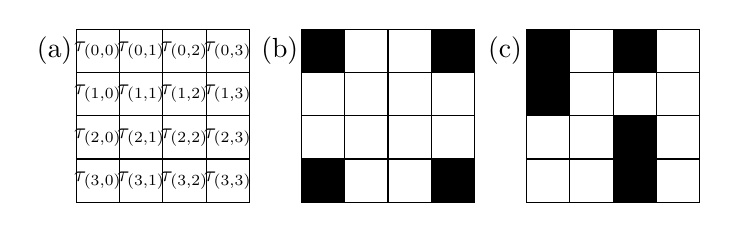
\begin{tikzpicture}[x=0.55cm, y=0.55cm] % {{{
\pgfmathsetmacro{\unitstep}{5.2}
\begin{scope}[shift={(0*\unitstep,0)}] % Coordenadas {{{
\node at (-0.5,0.5) {(a)} ;
    \foreach \x in {0,1,2,3} {
      \foreach \y in {0,1,2,3} {
        \begin{scope}[shift={(\x,-\y)}] 
          \draw (0,0) rectangle (1,1); 
          \node at (0.5,0.5) {\scalebox{.8}{$\tau_{(\y,\x)}$}};
         \end{scope}
%         \node at (0,-\y) (input\y) {$i_\y$};
%         \node[block] at (2,-\y) (block\y) {$f_\y$};
%         \draw[->] (input\y) -- (block\y);
%         \draw[->] (block\y.east) -- +(0.5,0);
    }
    }
\end{scope} % }}}
\begin{scope}[shift={(1*\unitstep,0)}] % Good channel {{{
\node at (-0.5,0.5) {(b)} ;
    \foreach \x in {0,1,2,3} {
      \foreach \y in {0,1,2,3} {
        \begin{scope}[shift={(\x,-\y)}] 
          \draw (0,0) rectangle (1,1); 
%           \node at (0.5,0.5) {$\tau_{\y,\x}$};
         \end{scope}
%         \node at (0,-\y) (input\y) {$i_\y$};
%         \node[block] at (2,-\y) (block\y) {$f_\y$};
%         \draw[->] (input\y) -- (block\y);
%         \draw[->] (block\y.east) -- +(0.5,0);
    }
    }
\begin{scope}[shift={(0,-3)}] \fill[black] (0,0) rectangle (1,1); \end{scope}
\begin{scope}[shift={(3,-3)}] \fill[black] (0,0) rectangle (1,1); \end{scope}
\begin{scope}[shift={(0,0)}] \fill[black] (0,0) rectangle (1,1); \end{scope}
\begin{scope}[shift={(3,0)}] \fill[black] (0,0) rectangle (1,1); \end{scope}
\end{scope} % }}}
\begin{scope}[shift={(2*\unitstep,0)}] % Good channel {{{
\node at (-0.5,0.5) {(c)} ;
    \foreach \x in {0,1,2,3} {
      \foreach \y in {0,1,2,3} {
        \begin{scope}[shift={(\x,-\y)}] 
          \draw (0,0) rectangle (1,1); 
%           \node at (0.5,0.5) {$\tau_{\y,\x}$};
         \end{scope}
%         \node at (0,-\y) (input\y) {$i_\y$};
%         \node[block] at (2,-\y) (block\y) {$f_\y$};
%         \draw[->] (input\y) -- (block\y);
%         \draw[->] (block\y.east) -- +(0.5,0);
    }
    }
\begin{scope}[shift={(0,0)}] \fill[black] (0,0) rectangle (1,1); \end{scope}
\begin{scope}[shift={(0,-1)}] \fill[black] (0,0) rectangle (1,1); \end{scope}
\begin{scope}[shift={(2,0)}] \fill[black] (0,0) rectangle (1,1); \end{scope}
\begin{scope}[shift={(2,-2)}] \fill[black] (0,0) rectangle (1,1); \end{scope}
\begin{scope}[shift={(2,-3)}] \fill[black] (0,0) rectangle (1,1); \end{scope}
\end{scope} % }}}
\end{tikzpicture} % }}}
	\caption{In (a) we introduce the
positions of two qubit diagrams. The diagrams in 
(b) corresponds to a quantum channel that results from the tensor product of
bit flip channels in each qubit [see \fref{fig:one:qubit:examples}(c)],
and in (c) a diagram of a map that is not a quantum channel is presented.}
	\label{fig:two:qubit:examples}
\end{figure} % }}}

% In \Fref{fig:PCE_figs} we introduce a pictorial representation of PCE operations of 
% 1, 2 and 3 qubits. Every position in the column, board or cube is associated with 
% the subindices of $\taus$ of a PCE operation. If a little square or cube  in position
% $\alpha_1,\ldots,\alpha_N$ is black, then $\taus=1$, if it is white, then $\taus=0$. For example,
% \begin{center}
% 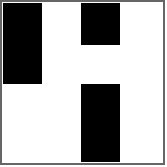
\includegraphics[width=2cm]{2qubits_pce_example}
% \end{center}
% this represents a PCE operation of 2 qubits that leaves invariant the Pauli 
% components $r_{0,0}$, $r_{0,2}$, $r_{1,0}$, $r_{2,2}$, $r_{3,2}$. This operation
% is not completely positive and therefore is not a quantum channel. In contrast, 
% \begin{center}
% \includegraphics[width=2cm]{2qubits_pceChannel_example01}
% \end{center}
% this other example of PCE operation that leaves invariant Pauli components 
% $r_{0,0}$, $r_{1,2}$, $r_{2,1}$, $r_{3,3}$ satisfies complete positivity and 
% is a quantum channel. 
% 
% \begin{figure} % {{{
% 	\centering
% 	\hfill \hfill
% 	\includegraphics[height=2.5cm]	{tablero_1qubit}
% 	\hfill
% 	\includegraphics[height=2.5cm]{tablero_2qubits}
% %	\hspace{1mm}
% %	\includegraphics[height=2.7cm]{rho-3q}
% 	\hfill \hfill \hfill
% 	\caption{From left to right representations of identity map
% 	(also PCE operations) of 1 and 2 qubits, respectively.}
% 	\label{fig:PCE_figs}
% \end{figure} % }}}
% 
% \begin{figure} % {{{
% 	\centering
% 	\includegraphics[height=2.5cm]	{1qubit_PCEChannels}
% 	\caption{1 qubit PCE channels. }
% 	\label{fig:1qubit_PCEChannles}
% \end{figure} % }}}



% }}}




